\chapter{Design and Implementation of the Proof-of-Concept Application}

Whereas the previous chapters were dedicated in providing a comprehensive literature
review on the topic, we will now focus on the practical implementations of integrating
solutions based on CRDTs in distributed software. In order to achieve this, we will
analyze a use case in which the implementation of CRDT-based data structures proves to be
\textit{valuable}, and document the development of a Proof-of-Concept application built
around that use case.
% TODO: replace the word valuable with something different 

\section{Defining the Use Case for the Proof-of-Concept}

The traditional infrastructure surrounding the broad family of collaborative applications
-- e.g., Google Docs, OneDrive, and many more -- have constantly relied on centralized
coordination paradigms, such as OT. While the approach of designating a central
coordinator for conflict resolution offers distinct advantages -- primarily revolving
around enabling near real-time, non-blocking collaboration and preserving the user's
intention -- there are some contexts in which centralization may present significant
drawbacks, mostly in terms of partition tolerance. For instance, the central coordinator
may be put in a position to be the single point of failure; if it is unreachable, there
is no other node that can approve or order changes, and the operativity of the entire
system collapses\footnote{Some countermeasures can be adopted, such as implementing a
leader election mechanism for designating a new central coordinator node among the nodes
of the network. Nevertheless, this approach would introduce a further layer of complexity
in the distributed system, and would require appropriate handling to enforce
convergence.}.

This precisely illustrates the fundamental advantage of decentralized, peer-to-peer (P2P)
architectures based on CRDTs; through replication across multiple nodes, information is
maintained with high availability and consistency -- i.e., compliant with SEC
constraints. Furthermore, if one or more nodes of the system fail, the system's
operativity is still guaranteed, as updates travel to all active nodes -- whereas the
faulty nodes will reconcile with the system's consistent state, once they come back
online. This approach eliminates the threat of a single point of failure that would
compromise system-wide reliability.

To illustrate this principle, we present a proof-of-concept implementation in the form of
a replicated file storage system that leverages CRDTs to achieve eventual consistency
without the need of centralized conflict resolution mechanisms. This system enables
multiple users to execute fundamental file operations -- including file sharing and
deletion -- on a shared storage infrastructure. 

Furthermore, the solution provides a \textit{file signature} mechanism, through which an
unique user provides a secure method of certifying its ownership over the same file, and
on-demand validity check over the signature can be requested by any other user.

In the following sections, we will refer to the proof-of-concept by the name of
\textit{CRDTSign}. 

\subsection{Proof-of-Concept Scope and Boundaries}

The primary objective that CRDTSign seeks to carry out in its current form is to
serve as a tangible illustration of the capabilities of CRDTs in contemporary
distributed peer-to-peer (P2P) systems. As such, several high-level requirements
must be satisfied:

\begin{itemize}
	\item consistent with the principles of decentralized applications, the backend
		logic is not centralized on a single node, but is served independently at each
		participating node;
	\item because CRDTSign aims to provide an example of modern collaborative software,
		convergence among nodes must be achieved in near real-time -- to satisfy end-user
		expectations for system responsiveness.
\end{itemize}

Conversely, given that the digital signature mechanism is integral to the solution --
serving as a certificate of ownership for files shared by users -- the system must adopt
a cryptographic signature scheme that ensures:

\begin{itemize}
	\item \textit{Integrity}: signatures cannot be altered without detection;
	\item \textit{Authenticity}: the signer's identity can be verified;
	\item \textit{Non-repudiation}: the signer cannot deny having signed the data.
\end{itemize}

As an additional requirement, the system adopts a data retention policy, which ensures
that files whose creation timestamp exceeds a configurable interval -- e.g., 90 days --
are automatically removed from the shared storage. This is made possible to prevent cases
in which the storage's memory becomes saturated over time by files which are unused or
obsolete.

It is worth underlining that the solution developed through CRDTSign poses itself as a
"toy" implementation. While it satisfies the core requirements illustrated above, certain
architectural constraints hinder its expectations of performance in production-grade
environments. For instance, the P2P architecture was not constructed from the ground up;
instead, it was abstracted through the use of a relay server. Rather than enabling direct
node-to-node communication, all messages are routed through the relay server, which in
turn broadcasts them to all peers -- thereby simulating a P2P environment. This design
choice does not fundamentally compromise the decentralized nature of the system, as
concurrency management logic remains managed across individual nodes, rather than being
centralized within the relay server. Additionally, the CRDT data structure was sourced
from an open-source library, and was not custom-made for this application. As we will
discuss in the next chapter, a more robust and scalable solution could be achieved by
designing a domain-specific CRDT structure and message exchange protocol tailored to the
characteristics of the shared data.

\subsection{User Stories}

We will now discuss several use cases of CRDTSign by describing the functionalities of
the system that are available to the end-user.

\paragraph{Uploading a file to storage}
Suppose that \textit{User A} has the need to share a file with a group of users -- e.g.,
\textit{User B} and \textit{User C}. To do so, it possesses a dedicated terminal
(\textit{Node A}), through which it can access CRDTSign's \textit{Web interface}. Once
connected and authenticated in the Web interface, User A uploads the file that it wants
to share to the storage; at this point, the system reads the file, and computes a digital
signature that uniquely identifies User A as the author of the uploaded file. Internally,
the system first adds the file to its local storage, saving its metadata accordingly, and
encapsulates the corresponding change to its state in an update message that is then
broadcast to all other active nodes. Conversely, both Nodes B and C receive the update, 
and autonomously apply it to their respective local storages. After the update is
successfully applied, both User B and User C can visualize the uploaded file and its
metadata in their respective Web interfaces, and can inspect it for further details.

\begin{figure}[tb!]
    \centering
    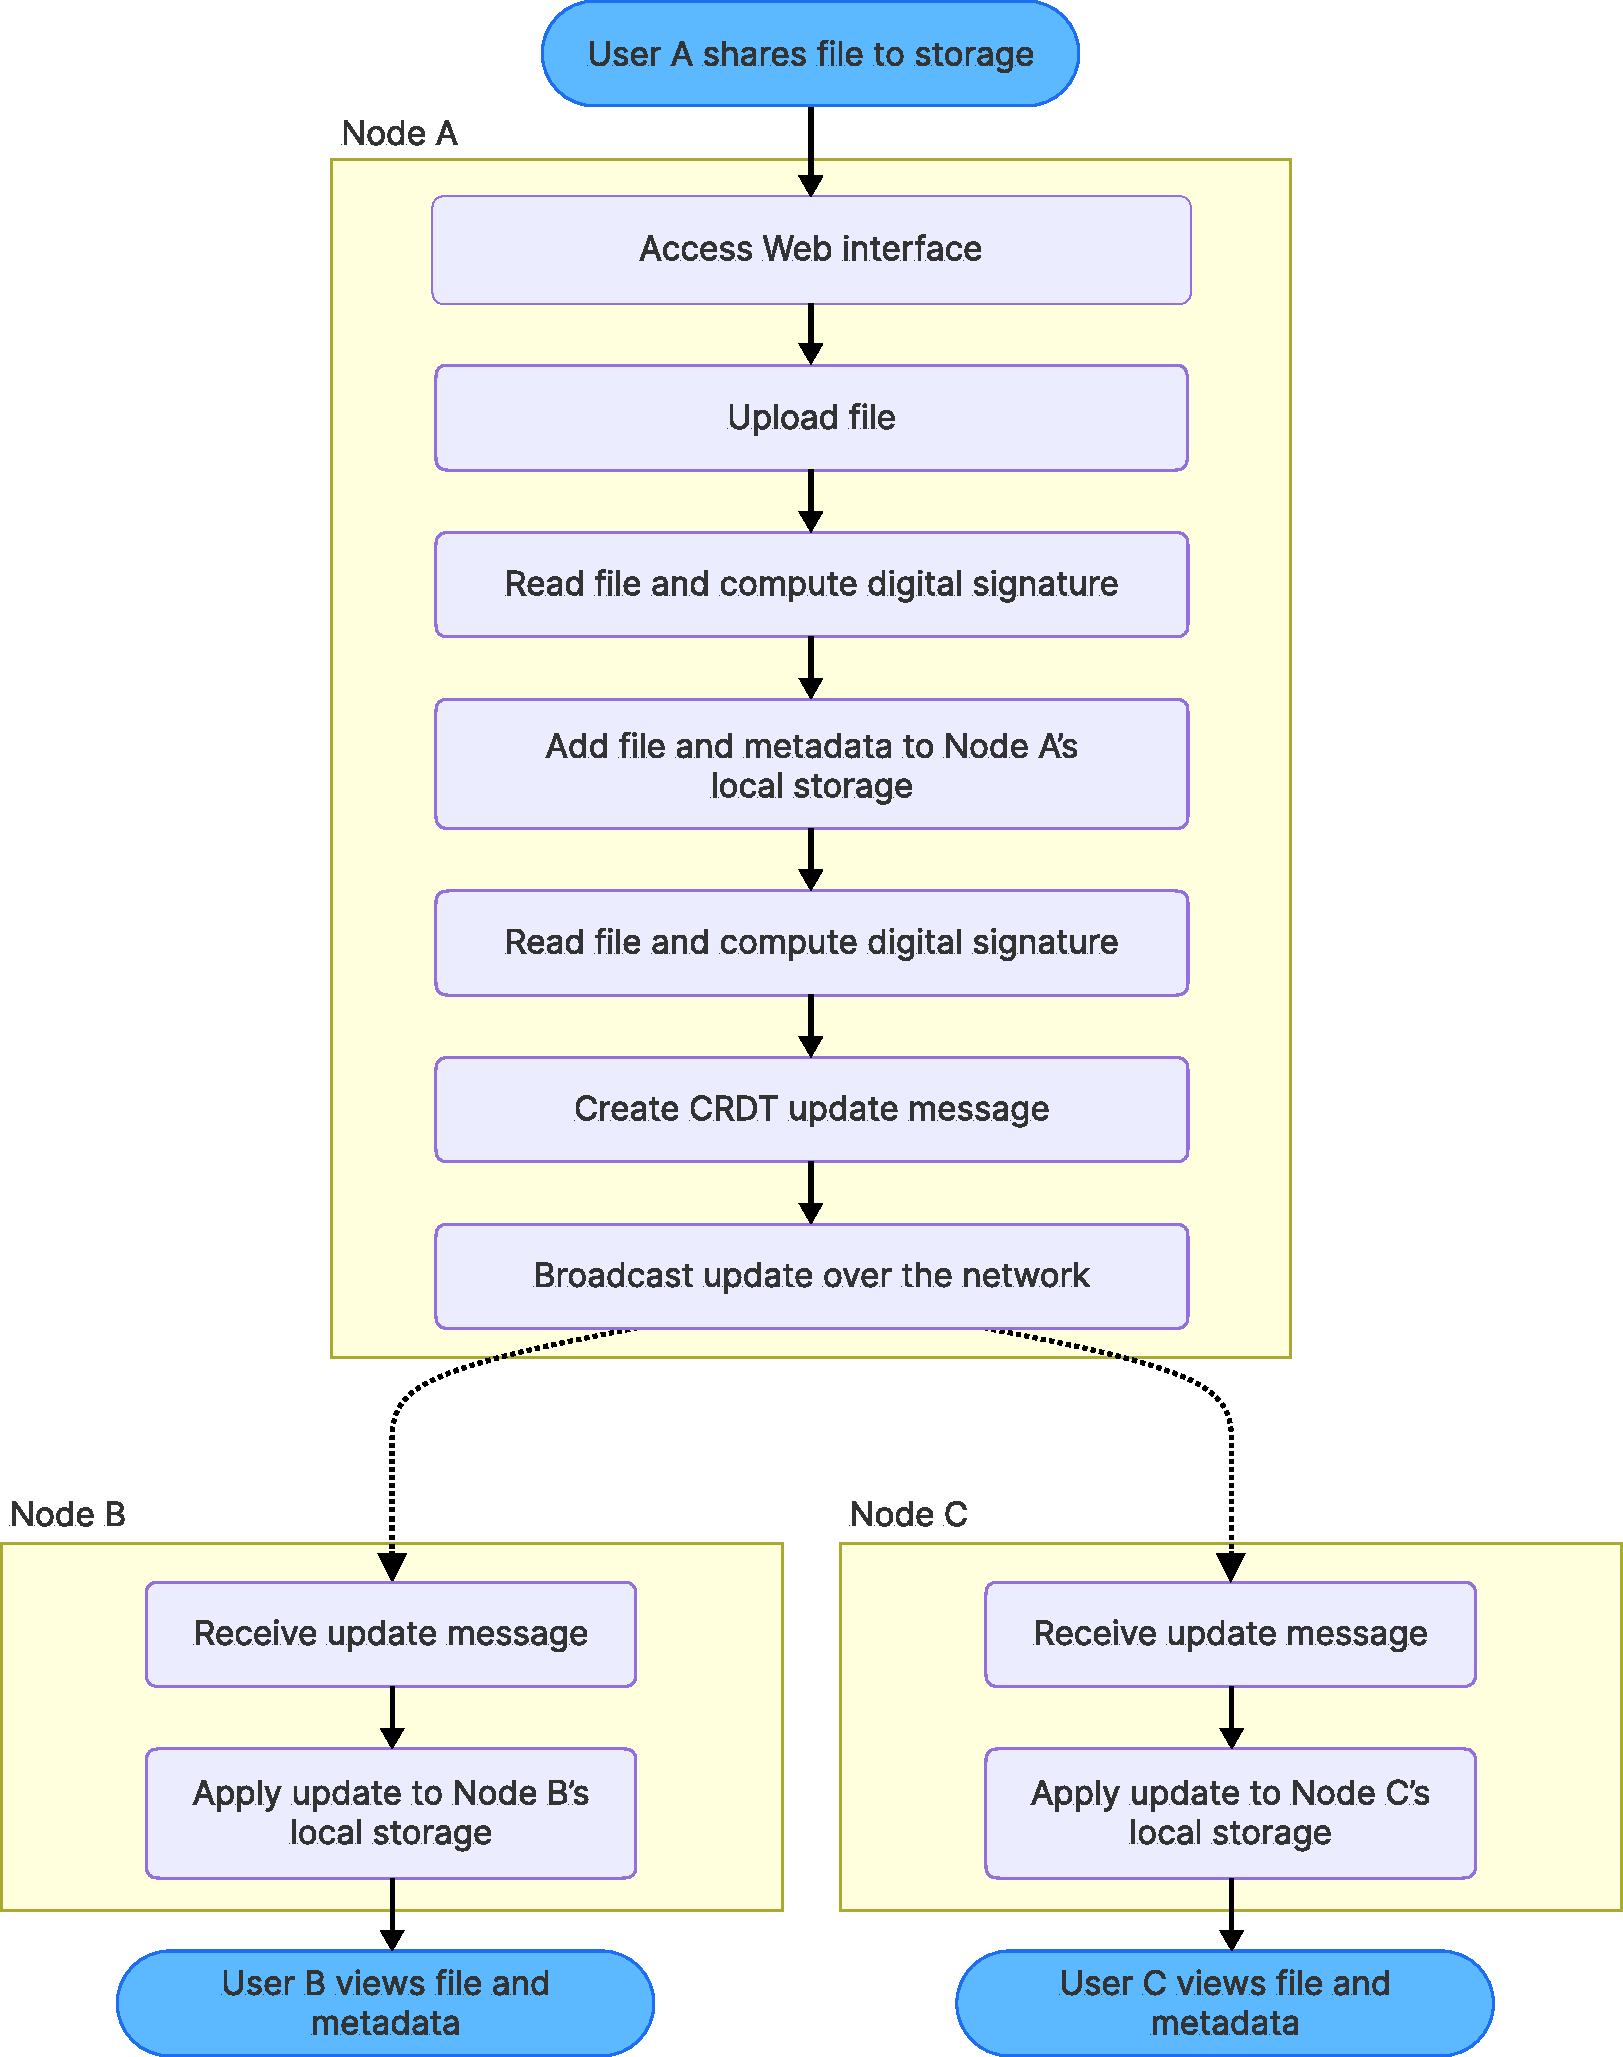
\includegraphics[width=0.8\linewidth]{diagram-file-upload.pdf}
    \caption{High-level flow diagram for the file upload procedure}
    \label{fig:diagram-file-upload}
\end{figure}

\paragraph{Verifying the validity of a file signature}
Suppose now that, once User B receives the file uploaded from User A, it wants to confirm
that the file was indeed uploaded by User A itself. To do so, it can request a
\textit{signature validity check} for the aforementioned file. Consequently, Node B
retrieves the file metadata, combines it with details concerning User A's identity --
i.e., User A's unique identifier -- and uses them to cryptographically validate the
signature to verify. Node B can either assert that the signature is valid, if the
check is successfull, or it is not valid, if the cryptographic validity check fails
with the given parameters. Finally, Node B informs the user -- through a notification
in the Web interface -- of the result of the signature validity check.

\begin{figure}[tb!]
    \centering
    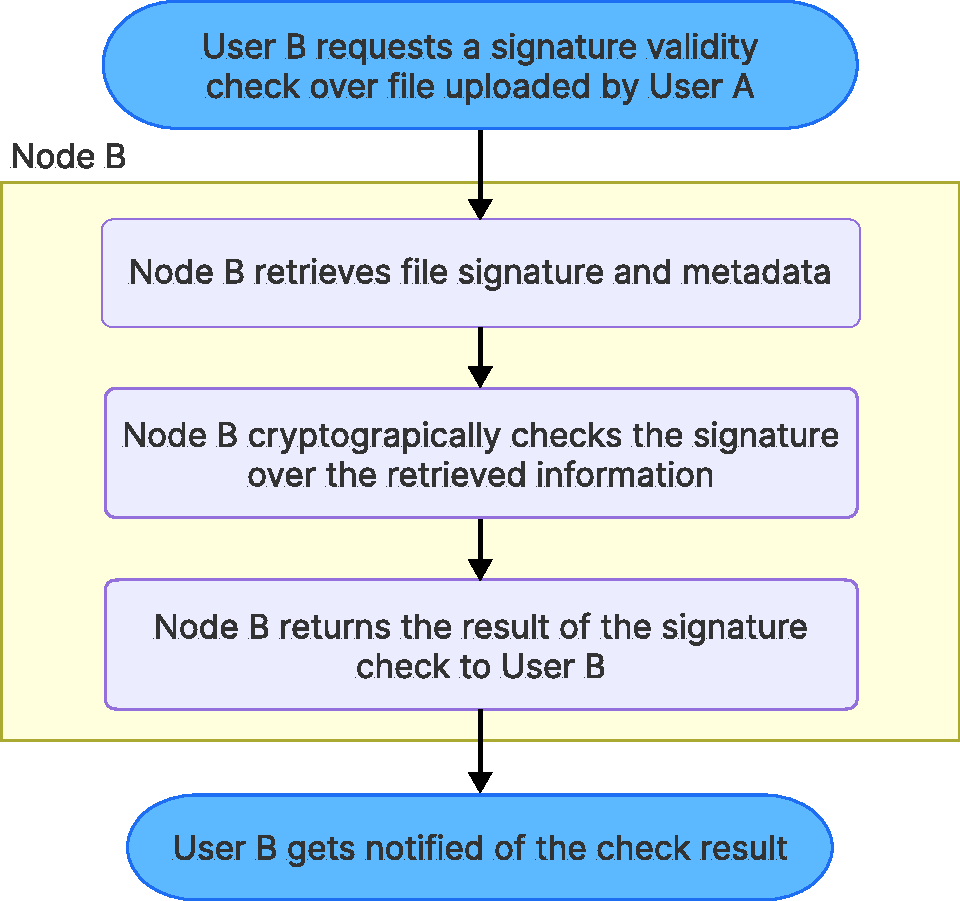
\includegraphics[width=0.61\linewidth]{diagram-signature-check.pdf}
    \caption{High-level flow diagram for the signature check procedure}
    \label{fig:diagram-signature-check}
\end{figure}

\paragraph{Deleting a file from storage}
Having received the file, User C seeks to remove it from storage\footnote{For the sake of
demonstration, whether User C decides to delete the file in agreement with other peers,
or of its own accord -- potentially exposing a malicious intent -- is irrelevant. In a
production-grade application, this can be easily addressed by implementing a
permission-based mechanism, which limits the set of actions a certain user can perform on
files uploaded by other users.}. It can do so by accessing the Web interface, selecting
the file in question, and request its removal from storage. The system responds by first
removing the file from local storage, and then computing an update message that reflects
the node's local state after the file removal. This update is then broadcast to all other
active nodes, which individually apply it to their respective local states -- leading to
a consistent state where the file is removed from storage. The procedure carries out
similarly to what occurs in \autoref{fig:diagram-file-upload}.

\section{System Architecture}

CRDTSign is made up of various components, each carrying out a specific task to achieve
the functionalities that were previously discussed. In the overall distribute network, we
can distinguish between two kinds of node:

\begin{itemize}
	\item \textit{Regular node}: is in charge of accepting and handling the user
		requests, employing both front-end and back-end logic. It is implemented through
		an application written in the
		\textit{Python}\footnote{https://www.python.org/} programming language,
		which exposes a Web interface through which all of CRDTSign's core
		functionalities are provided to the end-user. When triggered, each functionality
		invokes a custom-made Python library which implements and executes the back-end
		logic locally, interacting with suitable CRDT data structures when required.
		These structures are implemented through
		\textit{pycrdt}\footnote{https://y-crdt.github.io/pycrdt/}, a library that
		provides bindings to an open-source port of Yjs in the
		\textit{Rust}\footnote{https://rust-lang.org/} programming language.
	\item \textit{Relay node}: the server in charge of broadcasting messages to regular
		nodes. When a regular node sends an update to the relay node, the latter sends
		the corresponding message to all other nodes that need to receive it.
		Communication between regular nodes and the relay node occurs through the
		\textit{WebSocket} \cite{websocket_rfc} protocol.
\end{itemize}

\begin{figure}[h]
    \centering
    \includegraphics[width=0.61\linewidth]{diagram-system-architecture.pdf}
    \caption{Example of peer-to-peer communication through the relay node -- Node A
		delivers an update to the relay node, and the relay node delivers it to all other
		nodes}
    \label{fig:diagram-system-architecture}
\end{figure}


\section{Software Components}

This section describes the technical implementation of the software components that form
CRDTSign. The overall solution is organized in a modular fashion, and can be clustered
into three core elements, which are the \textit{back-end} engine, the \textit{front-end}
interface, and the \textit{relay server} logic. While the first two are equally deployed
at each individual node of the distributed network, the third is hosted by a dedicated
node belonging to the same network. Furthermore, the specifications of the chosen
digital signature scheme are illustrated, along with the design choices that were taken
to integrate such scheme in the solution.

\subsection{Back-end}

The back-end serves as the main computational engine for each node in the network. As
discussed above, the back-end logic is encapsulated through a custom-made library that
supports several core functionalities of the solution. We can distinguish among the
following operations.

\begin{itemize}
	\item User identity management (module \texttt{user.py})
	\item Cryptographic signature generation and validation (module \texttt{sign.py}).
	\item CRDT state management and persistence (module \texttt{storage.py}).
	\item Additional utility operations, such as file serialization and deserialization
		(module \texttt{file\_utils.py}), and operations concerning the enforcement of
		ad-hoc data retention policies (module \texttt{data\_retention.py}).
\end{itemize}

\subsubsection{\texttt{user.py} -- User identity management}

The \texttt{user.py} module curates the identity management and persistence on local
storage. The operations provided by this module ensure that all the necessary
information revolving the user connecting to the solution is correctly generated.
This information is then referenced when the user uploads a file through the
solution's front-end interface.

For instance, the following objects are associated to a user entity:
\begin{itemize}
	\item the user's \textit{unique identifier} (\texttt{user\_id}), which is generated by
		randomly selecting 12 alphanumeric charaters from the ASCII set -- which comprises
		both upper-case and lower-case variants of the 26 letters of the latin alphabet,
		and 10 digits from 0 to 9;
	\item the user's \textit{displayed name} (\texttt{username}), which is inputted by
		the user upon first login to the web interface.
\end{itemize}

Moreover, the module provides operations for handling the saving and loading operations
of the generated information into a dedicated file in local storage. Saved files are
placed in a location which is accessible to the \texttt{storage.py} module -- and as we
will see in \autoref{sec:frontend}, from the API interface.

All of the above operations are contained in a dedicated abstract class, named
\texttt{User}.

\subsubsection{\texttt{sign.py} -- Cryptographic signature generation and validation}

The \texttt{sign.py} module provides a collection of Python methods that enable the
system to generate suitable file signatures -- and consequently validate them on-demand.

Under the hood, the module leverages the \textit{Ed25519} scheme \cite{bernstein2011high}
for signature management, which is the primary implementation of the
\textit{Edwards-curve Digital Signature Algorithm} (EdDSA) -- based on the
\textit{SHA-512} hash function and the \textit{Curve25519} elliptic curve
\cite{eddsa_rfc}. The Python implementation of Ed25519 is provided by the open-source
\textit{cryptography} library\footonote{https://github.com/pyca/cryptography}.
Namely, the core payload of the Ed25519 implementation provided by this library is
a 64 byte-sized cryptographic keypair -- made up of a private and a public key, both
having a size of 32 bytes -- that can be associated to the specific user. The system
then uses the user's private key to \textit{sign} a given payload -- in this case,
the target file's \textit{SHA-256} hash digest was chosen to represent such payload.
The output of this process is a 64 byte signature, that can be then passed to the
\texttt{storage.py} module for attachment to the target file's metadata.

The module also provides a custom signature \textit{validation} method, which
requires three inputs:
\begin{itemize}
	\item the target file's \textit{hash digest};
	\item the target file's \textit{signature};
	\item the \textit{public key} associated to the target file's signing user.
\end{itemize}

The custom method uses the public key to verify the given signature over the file hash
that was used to generate the same signature, and returns a boolean output reflecting the
outcome of the verification -- \texttt{True} if the signature is deemed \textit{valid}
with the provided parameters, \texttt{False} otherwise.

\subsubsection{\texttt{storage.py} -- CRDT state management and persistence}

The \textit{storage.py} serves as the computational engine responsible for operations
executed on the available CRDT objects. On each node, two core objects are managed, each
within a dedicated abstract class: the \texttt{FileSignatureStorage} class and the
\texttt{UserStorage} class. These classes implement state management performed both
on the CRDT object they instantiate, and on the persisted data on local storage. For
instance, each performed CRDT operation -- \textit{add} or \textit{remove} -- triggers a
dump of the CRDT's current state to local storage. The system also checks at boot time
whether a state artifact is present in local storage, and loads it accordingly.

\paragraph{\texttt{FileSignatureStorage}}
The \texttt{FileSignatureStorage} class is employed to manage the files shared among
nodes in dedicated CRDTs modeled as key-value stores -- implemented using the
\textit{pycrdt} library's \texttt{Map} object. The key for each item in the CRDT is
the uploaded file's unique ID, while its corresponding value is a Python
\textit{dictionary} object which contains the following information:

\begin{itemize}
	\item the uploaded file's \textit{name};
	\item the uploaded file's \textit{hash digest};
	\item the uploaded file's \textit{signature} and its \textit{timestamp};
	\item information revolving the \textit{signing user} associated to the uploaded file
		-- \textit{display name} and \textit{unique ID}.
\end{itemize}

For convenience, the uploaded file is shared within the CRDT by preliminarily embedding
it in the metadata as a (serialized) \textit{file blob}. Details on the file blob
serialization and deserialization operations are illustrated in the next sub-section.
Upon retrieval of CRDT update containing the new file entry, if the node's back-end
identifies a file blob embedded in the metadata, it deserializes it and saves it to
local storage, and deletes the file blob from the metadata dictionary.

The metadata dictionary may also contain a timestamp indicating the expiration of the
file signature's validity. This element is optional, as the user can choose to input
it from the Web interface during the file upload process -- or leave it blank, which
indefinitely preserves the validity of the file signature itself.

An additional method is provided within the \texttt{FileSignatureStorage} class, which
regulates the custom \textit{data retention policy enforcement} routine, which triggers
each time the class is instantiated -- generally, this only occurs when the back-end
module is initially booted. The routine retrieves a configuration parameter that
indicates the data retention interval for newly uploaded files -- e.g., 90 days. For each
file in the CRDT, the routine constructs a synthetic timestamp ($t_{retention}$) by using
the file signature's timestamp, and offsetting it forwards by the retention interval
identified previously. This synthetic timestamp is then compared with the current timestamp
($t_{now}$), which leads to one of two possible scenarios:

\begin{itemize}
	\item if $t_{now} \geq t_{retention}$, this means that the file's retention has
		expired. Consequently, the file is removed from CRDT, and an update operation
		issued to all remote nodes.
	\item if $t_{now} < t_{retention}$, this means that the file's retention has not
		yet expired. No action is taken by the system in this case.
\end{itemize}

\paragraph{\texttt{UserStorage}}
Similar to what occurs for the \texttt{FileSignatureStorage} class, a dedicated CRDT
key-value store is reserved within the \texttt{UserStorage} class, to collect information
concerning the identities of registered users. For each user, an entry in the key-value
store is present -- with key equal to the given user's unique ID -- with a Python
dictionary attached to it containing the following user data.

\begin{itemize}
	\item the user's \textit{display name};
	\item the user's \textit{public key};
	\item the \textit{timestamp} associated to the registration of the user.
\end{itemize}

Fundamentally, the CRDT provided by this class is made available for quick access by any
signature validity check operation, as it may occur that a user requires verification for
a file shared by another user. By retrieving the signing user's unique ID, it can then
access the CRDT to obtain the correct public key to use in the validity check operation.

\paragraph{Interoperability with the relay server}
Both the \texttt{FileSignatureStorage} and the \texttt{UserStorage} classes require
connection with the relay server before any operation can be issued on their respective
CRDT structures. This is possible thanks to a dedicated library,
\textit{pycrdt-websocket}\footnote{https://github.com/y-crdt/pycrdt-websocket},
which extends the CRDT objects provided by the \textit{pycrdt} library with the
possibility of broadcasting CRDT updates to an available WebSocket server. Thus, during
their respective initialization phases, both the classes mentioned above start with a
blank CRDT key-value store, load the current state snapshot from local storage, if
available, and initiate a connection to a given IP address and port, which points to
the network's available relay server. If the connection is successful, the connected
CRDT object is saved within the newly initialized class object, ready to be used for
further operations. If the node fails to connect to the relay server over WebSocket,
the node continues to function in an "offline-only" fashion -- any operation issued
during this period will be broadcast on the next successful connection to the relay
server.

\subsubsection{\texttt{file\_utils.py} -- File blob serialization and deserialization}

File blobs that are placed in the CRDT key-value store employed by the
\texttt{FileSignatureStorage} class are subject to custom serialization and
deserialization procedures. For instance, the \textit{serialization} operation takes the
target file's binary data as input, and applies the open-source \textit{LZ4} compression
algorithm\footnote{https://lz4.org/} to the retrieved data. The output of the
compression algorithm is the payload that is embedded as the target file's blob in the
metadata saved inside the CRDT. Conversely, the \textit{deserialization} operation takes
the file's blob as input, and decompresses it via the same LZ4 algorithm, returning the
original file's content as output.

\subsection{Front-end}\label{sec:frontend}
CRDTSign's \textt{api.py} module serves as the user's entry point to the application. Its
main objective is to initialize an asynchronous RESTful API through the
\textit{Quart}\footnote{https://quart.palletsprojects.com/en/latest/#} framework.
Namely, the API instantiates several endpoints that can be accessed by interacting with
the components of the deployed Web application.

\paragraph{Root (\texttt{/})}
The main entry point to the application's user interface (UI). By accessing this endpoint
through a traditional Web browser, a dynamic HTML web page containing the UI is rendered
on the client's machine\footnote{The dynamic web page is constructed by parsing
pre-defined template files written using HTML syntax and special placeholders, which can
be read by the \textit{Jinja} templating engine for Python
(\url{https://jinja.palletsprojects.com/en/stable/})}.

\begin{figure}[tb!]
    \centering
    \includegraphics[width=\linewidth]{crdtsign-web-main.png}
    \caption{The main view for CRDTSign's front-end.}
    \label{fig:crdtsign-web-main}
\end{figure}

Upon the first access to the root endpoint -- performed by an un-registered user -- a new
\texttt{User} object is created with a unique ID, and a form is displayed on the UI where
the user can input the display name it wishes to appear under. After the user submits the
inserted display name, the web application's main view is displayed -- shown in
\autoref{fig:crdtsign-web-main}. The main view contains a table containing the signed
files that are present in the files CRDT storage; for each row of the table, the
following information is shown.

\begin{itemize}
	\item The signed file's \textit{name}.
	\item The signing user's \textit{display name}.
	\item The signature's \textit{creation timestamp}.
	\item The signature's \textit{expiration timestamp} -- if present.
	\item A set of \textit{action buttons}, named \textit{Details}, \textit{Validate},
		and \textit{Delete} respectively.
\end{itemize}

\begin{figure}[tb!]
    \centering
    \includegraphics[width=\linewidth]{crdtsign-web-details.png}
    \caption{An example of "Details" modal that displays information for a sample file.}
    \label{fig:crdtsign-web-details}
\end{figure}

The \textit{Details} button opens a modal which contains further details on the selected file, such as
the file's \textit{hash digest}, its \textit{signature}, and all the information mentioned above. An
example of the modal being displayed can be found in \autoref{fig:crdtsign-web-details}

\begin{figure}[tb!]
    \centering
    \includegraphics[width=\linewidth]{crdtsign-web-validate.png}
    \caption{The user is notified that the checked file signature is valid.}
    \label{fig:crdtsign-web-validate}
\end{figure}

The \textit{Validate} button issues a request to check the validity of the selected
file's signature. This request is dispatched to the back-end using the available
methods, and the outcome of the check is then displayed in a pop-up notification
appearing in the top-right corner of the web browser -- as shown in
\autoref{fig:crdtsign-web-validate}. If present, the user is also informed of the
signature's validity expiration -- date and time.

The \textit{Delete} button is used to request the removal of the selected file. After
further confirmation to proceeed with the operation is submitted by the user, a
\textit{delete} operation is issued on the local CRDT, which then broadcasts it to all of
the remote nodes.

\begin{figure}[tb!]
    \centering
    \includegraphics[width=\linewidth]{crdtsign-web-sign.png}
    \caption{The form used to upload a new file to storage.}
    \label{fig:crdtsign-web-sign}
\end{figure}

Furthermore, the main view presents a set of tab buttons that link to additional views.
Namely, the \textit{"Sign File"} view -- \autoref{fig:crdtsign-web-sign} -- displays a
form that allows the user to upload a new file to be signed and preserved in CRDT
storage, and specify additional information, such as the date and the time of the
signature's validity expiration.

\paragraph{Retrieve/upload files (\texttt{/api/signatures})}
The endpoint that is linked to the signed files CRDT storage. Files can be retrieved
cumulatively or selectively -- if a file ID is specified in the request -- or uploaded
and signed via a \texttt{POST} request to the same endpoint. A request to remove a given
file can also be performed on this endpoint via a \texttt{DELETE} request, by passing the
target file's ID (\texttt{<file\_id>}).

\paragraph{Validate file signature (\texttt{/api/validate/<file\_id>})}
The endpoint used to request a validity check for the file denoted by the passed ID
(\texttt{<file\_id>}) and returns the outcome of such check.

\subsection{Relay Server}
The solution's relay server is used to emulate a pure-P2P environment among the nodes of
the network. Its sole purpose is to keep track of connections that each node entertains
with the server itself over the WebSocket protocol, and broadcast incoming CRDT update
messages to the interested nodes. This is done by leveraging the \textit{pycrdt} and
\textit{pycrdt-websocket} libraries, and using the latter library's \texttt{Store}
object to keep a record of incoming update messages. This persistence mechanism is useful
for synchronization purposes, as it enables a  newly-connected node -- or a known node
that has suffered a given period of downtime -- to be brought up to date with the current
state of CRDT objects.

The relay server instantiates a set of \textit{rooms}, each one being a container for a
shared object. This means that each backend has to be routed to the correct room -- one
for the shared files, and one for the registered users -- in order to share changes
applied to the same objects.

The underlying relay server logic is then made accessible to a known IP address and port
the solution's local network by using the open-source
\textit{Hypercorn}\footnote{https://hypercorn.readthedocs.io/en/latest/} library,
which is used to deploy a standalone web server based on the
ASGI\footnote{https://github.com/django/asgiref/blob/main/specs/asgi.rst}
(Asynchronous Server Gateway Interface) standard.

\section{Production Deployment}

Although CRDTSign's software architecture is sub-optimal with respect to
readiness for production environments, a few considerations have been made to better suit
the deployment of the entire solution.

For instance, the Python package that contains the software components described above
was built using the open-source \textit{uv}\footnote{https://docs.astral.sh/uv/}
package manager, which allowed for a seamless and efficient management of the required
Python dependencies and of the build environment.

The solution then uses the popular containerization engine
\textit{Docker}\footnote{https://www.docker.com/} create lightweight, standalone
containers used to deploy software components individually.

\section{Development of the Complementary Mobile Application}

As an addendum to the provided solution, a prototype mobile front-end application was
developed to wrap around the present back-end logic. The application was written using
the \textit{Flet} framework\footnote{https://flet.dev/}, which offers a simple
environment for building mobile and web applications, using Python syntax to construct
user interfaces. Software that is developed with Flet can be compiled using Flet's
custom build system, which translates it into code that is supported by the open-source
UI software development kit \textit{Flutter}\footnote{https://flutter.dev/}.
Flutter's capabilities are then leveraged to generate a package that can be executed --
or installed -- on a wide variety of devices -- i.e., desktop operating systems such as
Windows, Linux, or macOS, or mobile operating systems such as Android or iOS.

Through Flet, an application was developed -- named \texttt{crdtsign-mobile}, for
distinction with the main application -- to mimic the functionalities that are already
present in the main front-end application described in \autoref{sec:frontend}. Namely,
the mobile application is divided into two principal views that the user can navigate
between:

\begin{figure}[tb]
    \centering
    \begin{subfigure}[b]{0.45\textwidth}
        \centering
        \includegraphics[width=\textwidth]{crdtsign-mobile-home.png}
        \caption{A screenshot of the \textit{"home" view} for the CRDTSign mobile
			application.}
        \label{fig:crdtsign-mobile-home}
    \end{subfigure}
    \hfill
    \begin{subfigure}[b]{0.45\textwidth}
        \centering
        \includegraphics[width=\textwidth]{crdtsign-mobile-create.png}
        \caption{A screenshot of the \textit{"create" view} for the CRDTSign mobile
			application.}
        \label{fig:crdtsign-mobile-create}
    \end{subfigure}
\end{figure}

\begin{itemize}
	\item a \textit{"home"} view -- \autoref{fig:crdtsign-mobile-home} -- where the user
		can explore the available signed files from CRDT storage, and for each perform a
		common set of actions, such as viewing relevant details for a file, requesting a
		validity check for a file, or remove a file from shared storage;
	\item a \textit{"create"} view -- \autoref{fig:crdtsign-mobile-create} -- where the
		user can upload a file to be signed and shared within the shared storage.
\end{itemize}
